% Author: Izaak Neutelings (June 2020)
% Inspiration: https://tex.stackexchange.com/questions/285578/how-to-draw-parallelepiped-and-cube-with-latex/288101#288101
\documentclass[border=3pt,tikz]{standalone}
\usepackage{amsmath}
\usepackage{physics}
\usepackage{siunitx}
\usepackage{xcolor}
\usepackage{etoolbox} %ifthen
\usepackage[outline]{contour} % glow around text
\usetikzlibrary{arrows.meta}
%\usetikzlibrary{calc}
%\usetikzlibrary{decorations.markings}
%\usetikzlibrary{angles,quotes} % for pic (angle labels)
\tikzset{>=latex} % for LaTeX arrow head
\contourlength{1.6pt}

\colorlet{myblue}{blue!70!black}
\colorlet{mydarkblue}{blue!40!black}
\colorlet{mygreen}{green!60!black}
\colorlet{myred}{red!65!black}
\colorlet{mypurple}{red!50!blue!95!black!75}
\colorlet{xcol}{blue!85!black}
\colorlet{vcol}{green!70!black}
\colorlet{projcol}{vcol!90!black!60}
\tikzstyle{wave}=[myblue,thick]
\tikzstyle{xline}=[very thick,myblue]
%\tikzstyle{vline}=[very thick,mygreen]
%\tikzstyle{aline}=[very thick,mypurple]
\tikzstyle{vector}=[->,very thick,vcol,line cap=round]
\tikzstyle{mydashed}=[green!30!black!90,dash pattern=on 2pt off 2pt,very thin]
\tikzstyle{mymeas}=[{Latex[length=3,width=2]}-{Latex[length=3,width=2]},thin]

\def\tick#1#2{\draw[thick] (#1) ++ (#2:0.05*\ymax) --++ (#2-180:0.1*\ymax)}

\begin{document}


% POSITION - MONKEY vs. DART
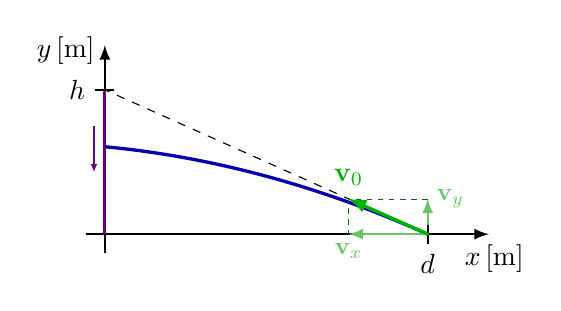
\begin{tikzpicture}
  \def\slope{0.65}
  \def\xmax{4.6}
  \def\ymax{2.4}
  \def\a{4.1}
  \def\c{-2.2}
  \def\v{1.1}
  \def\h{-\A*(2*\a-\c)*\a}
  \def\A{0.043}
  \def\nsamples{100}
  \coordinate (G) at (\a,0);
  
  % AXES
  \draw[->,thick]
    (-0.1*\ymax,0) -- (1.06*\xmax,0) node[right=2,below] {$x$\,[m]};
  \draw[->,thick]
    (0,-0.1*\ymax) -- (0,\ymax) node[below=2,left=0] {$y$\,[m]};
  
  % LINES
  \draw[dashed] (G) -- (0,{\A*(2*\a-\c)*\a}) coordinate (M);
  \draw[xline,variable=\x,samples=\nsamples,smooth,domain=0:\a]
    plot(\x,{-\A*(\x-\c+\a)*(\x-\a)});
  \draw[very thick,xcol!60!red] (0,{-\h}) -- (0,0);
  \draw[-{Latex[length=3,width=2.5]},xcol!60!red] (-0.03*\xmax,{-0.75*\h}) --++ (0,{0.32*\h});
  
  % VELOCITY
  \draw[->,projcol,thick]
    (G) --++ (0,{-\h*\v/sqrt(\a*\a+\h*\h)}) node[scale=0.9,right=0] {$\vb{v}_y$} coordinate (VY);
  \draw[->,projcol,thick]
    (G) --++ ({-\a*\v/sqrt(\a*\a+\h*\h)},0) node[scale=0.9,below=0] {$\vb{v}_x$} coordinate (VX);
  \draw[mydashed] (VY) -| (VX);
  \tick{G}{90} node[below] {$d$};
  \tick{M}{ 0} node[left] {$h$};
  \draw[vector,vcol] (G) --++ ({atan2(\h,\a)-180}:\v) node[above=1] {$\vb{v}_0$};
  
\end{tikzpicture}


% Y POSITION - MONKEY vs. DART PARABOLA
\def\xmax{3.6}
\def\ymax{2.4}
\def\nsamples{100}
\def\A{0.1}
\def\h{0.77*\ymax}
\def\d{1.8*\xmax}
\begin{tikzpicture}
  
  \draw[->,thick]
    (-0.1*\ymax,0) -- (1.06*\xmax,0) node[below] {$t$\,[s]};
  \draw[->,thick]
    (0,-0.1*\ymax) -- (0,\ymax) node[below=4,left=0] {$y$\,[m]};
  \draw[xline,very thick,xcol!60!red,variable=\t,samples=\nsamples,smooth,domain=0:0.9*\xmax]
    plot(\t,\h-\A*\t*\t) node[below=2,right] {$y_\mathrm{m}$};
  \draw[xline,very thick,xcol,variable=\t,samples=\nsamples,smooth,domain=0:0.9*\xmax]
    plot(\t,{-\A*\t*(\t-\d)}) node[right] {$y_\mathrm{d}$};
  
  \draw[dashed] ({\h/(\A*\d)},0) coordinate (T) --++ (0,0.84*\ymax);
  \draw[thick] (0.1,\h) --++ (-0.2,0) node[left] {$h$};
  \draw[thick] (T)++(0,0.1) --++ (0,-0.2) node[below] {$t_1$};
  
\end{tikzpicture}


% X POSITION - MONKEY vs. DART PARABOLA
\begin{tikzpicture}
  \draw[->,thick]
    (-0.1*\ymax,0) -- (1.06*\xmax,0) node[below] {$t$\,[s]};
  \draw[->,thick]
    (0,-0.1*\ymax) -- (0,\ymax) node[below=4,left=0] {$x$\,[m]};
  \draw[xline,very thick,xcol!60!red]
    (0,0) -- (0.9*\xmax,0) node[midway,left=6,above=-1] {$x_\mathrm{m}$};
  \draw[xline,very thick,xcol]
    (0,\h) -- ({\h/(\A*\d)},0) node[midway,above right=-3] {$x_\mathrm{d}$};
  \draw[dashed] ({\h/(\A*\d)},0) coordinate (T) --++ (0,0.84*\ymax);
  \draw[thick] (0.1,\h) --++ (-0.2,0) node[left] {$d$};
  \draw[thick] (T)++(0,0.1) --++ (0,-0.2) node[below] {$t_1$};
\end{tikzpicture}


\end{document}